% Options for packages loaded elsewhere
\PassOptionsToPackage{unicode}{hyperref}
\PassOptionsToPackage{hyphens}{url}
%
\documentclass[
]{article}
\usepackage{lmodern}
\usepackage{amssymb,amsmath}
\usepackage{ifxetex,ifluatex}
\ifnum 0\ifxetex 1\fi\ifluatex 1\fi=0 % if pdftex
  \usepackage[T1]{fontenc}
  \usepackage[utf8]{inputenc}
  \usepackage{textcomp} % provide euro and other symbols
\else % if luatex or xetex
  \usepackage{unicode-math}
  \defaultfontfeatures{Scale=MatchLowercase}
  \defaultfontfeatures[\rmfamily]{Ligatures=TeX,Scale=1}
\fi
% Use upquote if available, for straight quotes in verbatim environments
\IfFileExists{upquote.sty}{\usepackage{upquote}}{}
\IfFileExists{microtype.sty}{% use microtype if available
  \usepackage[]{microtype}
  \UseMicrotypeSet[protrusion]{basicmath} % disable protrusion for tt fonts
}{}
\makeatletter
\@ifundefined{KOMAClassName}{% if non-KOMA class
  \IfFileExists{parskip.sty}{%
    \usepackage{parskip}
  }{% else
    \setlength{\parindent}{0pt}
    \setlength{\parskip}{6pt plus 2pt minus 1pt}}
}{% if KOMA class
  \KOMAoptions{parskip=half}}
\makeatother
\usepackage{xcolor}
\IfFileExists{xurl.sty}{\usepackage{xurl}}{} % add URL line breaks if available
\IfFileExists{bookmark.sty}{\usepackage{bookmark}}{\usepackage{hyperref}}
\hypersetup{
  pdftitle={MPM Group Project - AirBnb Price Prediction},
  pdfauthor={Giedo, Micha, Azher, Christoph},
  hidelinks,
  pdfcreator={LaTeX via pandoc}}
\urlstyle{same} % disable monospaced font for URLs
\usepackage[margin=1in]{geometry}
\usepackage{color}
\usepackage{fancyvrb}
\newcommand{\VerbBar}{|}
\newcommand{\VERB}{\Verb[commandchars=\\\{\}]}
\DefineVerbatimEnvironment{Highlighting}{Verbatim}{commandchars=\\\{\}}
% Add ',fontsize=\small' for more characters per line
\usepackage{framed}
\definecolor{shadecolor}{RGB}{248,248,248}
\newenvironment{Shaded}{\begin{snugshade}}{\end{snugshade}}
\newcommand{\AlertTok}[1]{\textcolor[rgb]{0.94,0.16,0.16}{#1}}
\newcommand{\AnnotationTok}[1]{\textcolor[rgb]{0.56,0.35,0.01}{\textbf{\textit{#1}}}}
\newcommand{\AttributeTok}[1]{\textcolor[rgb]{0.77,0.63,0.00}{#1}}
\newcommand{\BaseNTok}[1]{\textcolor[rgb]{0.00,0.00,0.81}{#1}}
\newcommand{\BuiltInTok}[1]{#1}
\newcommand{\CharTok}[1]{\textcolor[rgb]{0.31,0.60,0.02}{#1}}
\newcommand{\CommentTok}[1]{\textcolor[rgb]{0.56,0.35,0.01}{\textit{#1}}}
\newcommand{\CommentVarTok}[1]{\textcolor[rgb]{0.56,0.35,0.01}{\textbf{\textit{#1}}}}
\newcommand{\ConstantTok}[1]{\textcolor[rgb]{0.00,0.00,0.00}{#1}}
\newcommand{\ControlFlowTok}[1]{\textcolor[rgb]{0.13,0.29,0.53}{\textbf{#1}}}
\newcommand{\DataTypeTok}[1]{\textcolor[rgb]{0.13,0.29,0.53}{#1}}
\newcommand{\DecValTok}[1]{\textcolor[rgb]{0.00,0.00,0.81}{#1}}
\newcommand{\DocumentationTok}[1]{\textcolor[rgb]{0.56,0.35,0.01}{\textbf{\textit{#1}}}}
\newcommand{\ErrorTok}[1]{\textcolor[rgb]{0.64,0.00,0.00}{\textbf{#1}}}
\newcommand{\ExtensionTok}[1]{#1}
\newcommand{\FloatTok}[1]{\textcolor[rgb]{0.00,0.00,0.81}{#1}}
\newcommand{\FunctionTok}[1]{\textcolor[rgb]{0.00,0.00,0.00}{#1}}
\newcommand{\ImportTok}[1]{#1}
\newcommand{\InformationTok}[1]{\textcolor[rgb]{0.56,0.35,0.01}{\textbf{\textit{#1}}}}
\newcommand{\KeywordTok}[1]{\textcolor[rgb]{0.13,0.29,0.53}{\textbf{#1}}}
\newcommand{\NormalTok}[1]{#1}
\newcommand{\OperatorTok}[1]{\textcolor[rgb]{0.81,0.36,0.00}{\textbf{#1}}}
\newcommand{\OtherTok}[1]{\textcolor[rgb]{0.56,0.35,0.01}{#1}}
\newcommand{\PreprocessorTok}[1]{\textcolor[rgb]{0.56,0.35,0.01}{\textit{#1}}}
\newcommand{\RegionMarkerTok}[1]{#1}
\newcommand{\SpecialCharTok}[1]{\textcolor[rgb]{0.00,0.00,0.00}{#1}}
\newcommand{\SpecialStringTok}[1]{\textcolor[rgb]{0.31,0.60,0.02}{#1}}
\newcommand{\StringTok}[1]{\textcolor[rgb]{0.31,0.60,0.02}{#1}}
\newcommand{\VariableTok}[1]{\textcolor[rgb]{0.00,0.00,0.00}{#1}}
\newcommand{\VerbatimStringTok}[1]{\textcolor[rgb]{0.31,0.60,0.02}{#1}}
\newcommand{\WarningTok}[1]{\textcolor[rgb]{0.56,0.35,0.01}{\textbf{\textit{#1}}}}
\usepackage{graphicx,grffile}
\makeatletter
\def\maxwidth{\ifdim\Gin@nat@width>\linewidth\linewidth\else\Gin@nat@width\fi}
\def\maxheight{\ifdim\Gin@nat@height>\textheight\textheight\else\Gin@nat@height\fi}
\makeatother
% Scale images if necessary, so that they will not overflow the page
% margins by default, and it is still possible to overwrite the defaults
% using explicit options in \includegraphics[width, height, ...]{}
\setkeys{Gin}{width=\maxwidth,height=\maxheight,keepaspectratio}
% Set default figure placement to htbp
\makeatletter
\def\fps@figure{htbp}
\makeatother
\setlength{\emergencystretch}{3em} % prevent overfull lines
\providecommand{\tightlist}{%
  \setlength{\itemsep}{0pt}\setlength{\parskip}{0pt}}
\setcounter{secnumdepth}{-\maxdimen} % remove section numbering

\title{MPM Group Project - AirBnb Price Prediction}
\author{Giedo, Micha, Azher, Christoph}
\date{4/25/2021}

\begin{document}
\maketitle

\hypertarget{description-of-the-project}{%
\section{Description of the Project}\label{description-of-the-project}}

In this report, our group analyses the influence of different predictors
on the listing price of AirBnb offerings in different cites in the
United States.

The final model should provide a way to estimate the correct price for
any new or existing object listed on AirBnB in order to ensure high
booking rates. Also, it ensures users of this model to not underprice
their object and lose out on improved margins. Please keep in mind, this
model does not take into consideration the exact location or `cleanness'
of an object due to a lack of data. However, both of these predictors
would have a high influence. Meaning, you apartment most likely still
needs to be clean to result in a high booking rate.

\hypertarget{data-preparation}{%
\section{Data Preparation}\label{data-preparation}}

As a first step, we load the data from our source .csv file and set all
categorical values to be considered as factors. We also load the
packages required to execute all our functions and calculations.

\hypertarget{data-understanding-data-analysis}{%
\section{Data Understanding / Data
Analysis}\label{data-understanding-data-analysis}}

Now we will take a deeper look at our data, the response variable
log\_price and all the available predictors.

Lets look at all the predictors of our data set.

\begin{Shaded}
\begin{Highlighting}[]
\KeywordTok{colnames}\NormalTok{(df.airbnb)}
\end{Highlighting}
\end{Shaded}

\begin{verbatim}
##  [1] "id"                     "log_price"              "property_type"         
##  [4] "room_type"              "accommodates"           "bathrooms"             
##  [7] "bed_type"               "cancellation_policy"    "cleaning_fee"          
## [10] "city"                   "host_has_profile_pic"   "host_identity_verified"
## [13] "instant_bookable"       "number_of_reviews"      "review_scores_rating"  
## [16] "bedrooms"               "beds"                   "amenities_Gym"         
## [19] "amenities_WiFi"         "amenities_Pets"         "amenities_Breakfast"
\end{verbatim}

We can see, our data set consists of a response variable and 19
predictors. The column name With a few simple commands, a better
understanding of the values can be gained.

\begin{Shaded}
\begin{Highlighting}[]
\KeywordTok{head}\NormalTok{(df.airbnb)}
\end{Highlighting}
\end{Shaded}

\begin{verbatim}
##         id log_price property_type room_type accommodates bathrooms bed_type
## 1  6901257  5.010635             0         0            3         1        4
## 2  6304928  5.129899             0         0            7         1        4
## 3  7919400  4.976734             0         0            5         1        4
## 4 13418779  6.620073            17         0            4         1        4
## 5  3808709  4.744932             0         0            2         1        4
## 6 12422935  4.442651             0         1            2         1        4
##   cancellation_policy cleaning_fee city host_has_profile_pic
## 1                   2            1    4                    1
## 2                   2            1    4                    1
## 3                   1            1    4                    1
## 4                   0            1    5                    1
## 5                   1            1    2                    1
## 6                   2            1    5                    1
##   host_identity_verified instant_bookable number_of_reviews
## 1                      1                0                 2
## 2                      0                1                 6
## 3                      1                1                10
## 4                      1                0                 0
## 5                      1                1                 4
## 6                      1                1                 3
##   review_scores_rating bedrooms beds amenities_Gym amenities_WiFi
## 1                  100        1    1             0              1
## 2                   93        3    3             0              1
## 3                   92        1    3             0              1
## 4                   94        2    2             0              1
## 5                   40        0    1             0              1
## 6                  100        1    1             0              1
##   amenities_Pets amenities_Breakfast
## 1              0                   0
## 2              0                   0
## 3              0                   1
## 4              0                   0
## 5              0                   0
## 6              0                   0
\end{verbatim}

Head provides an overview over the first 5 entries in the table, this
provides us with some knowledge about how the rows look.

\begin{Shaded}
\begin{Highlighting}[]
\KeywordTok{summary}\NormalTok{(df.airbnb)}
\end{Highlighting}
\end{Shaded}

\begin{verbatim}
##        id             log_price     property_type   room_type  accommodates  
##  Min.   :     344   Min.   :2.303   0      :48609   0:41017   Min.   : 1.00  
##  1st Qu.: 6255815   1st Qu.:4.317   17     :16424   1:30317   1st Qu.: 2.00  
##  Median :12252055   Median :4.718   11     : 2649   2: 2136   Median : 2.00  
##  Mean   :11262636   Mean   :4.783   28     : 1683             Mean   : 3.16  
##  3rd Qu.:16396710   3rd Qu.:5.220   22     : 1236             3rd Qu.: 4.00  
##  Max.   :21230903   Max.   :7.600   23     :  600             Max.   :16.00  
##                                     (Other): 2269                            
##    bathrooms     bed_type  cancellation_policy cleaning_fee city     
##  Min.   :0.000   0:  468   0:22338             0:19474      0: 3457  
##  1st Qu.:1.000   1:  265   1:18916             1:53996      1: 3714  
##  Median :1.000   2:  742   2:32092                          2: 5660  
##  Mean   :1.194   3:  577   3:  107                          3:22268  
##  3rd Qu.:1.000   4:71418   4:   17                          4:31975  
##  Max.   :8.000                                              5: 6396  
##                                                                      
##  host_has_profile_pic host_identity_verified instant_bookable number_of_reviews
##  0:  224              0:24006                0:54150          Min.   :  0.00   
##  1:73246              1:49464                1:19320          1st Qu.:  1.00   
##                                                               Median :  6.00   
##                                                               Mean   : 20.88   
##                                                               3rd Qu.: 23.00   
##                                                               Max.   :605.00   
##                                                                                
##  review_scores_rating    bedrooms           beds        amenities_Gym
##  Min.   : 20.00       Min.   : 0.000   Min.   : 0.000   0:66038      
##  1st Qu.: 93.00       1st Qu.: 1.000   1st Qu.: 1.000   1: 7432      
##  Median : 94.00       Median : 1.000   Median : 1.000                
##  Mean   : 94.06       Mean   : 1.267   Mean   : 1.713                
##  3rd Qu.: 99.00       3rd Qu.: 1.000   3rd Qu.: 2.000                
##  Max.   :100.00       Max.   :10.000   Max.   :18.000                
##                                                                      
##  amenities_WiFi amenities_Pets amenities_Breakfast
##  0: 2778        0:63352        0:65222            
##  1:70692        1:10118        1: 8248            
##                                                   
##                                                   
##                                                   
##                                                   
## 
\end{verbatim}

The summary() command provides a first statistical overview of the data.

\begin{Shaded}
\begin{Highlighting}[]
\KeywordTok{str}\NormalTok{(df.airbnb)}
\end{Highlighting}
\end{Shaded}

\begin{verbatim}
## 'data.frame':    73470 obs. of  21 variables:
##  $ id                    : int  6901257 6304928 7919400 13418779 3808709 12422935 11825529 13971273 180792 5385260 ...
##  $ log_price             : num  5.01 5.13 4.98 6.62 4.74 ...
##  $ property_type         : Factor w/ 19 levels "0","1","2","3",..: 1 1 1 13 1 1 1 8 13 13 ...
##  $ room_type             : Factor w/ 3 levels "0","1","2": 1 1 1 1 1 2 1 1 2 2 ...
##  $ accommodates          : int  3 7 5 4 2 2 3 2 2 2 ...
##  $ bathrooms             : int  1 1 1 1 1 1 1 1 1 1 ...
##  $ bed_type              : Factor w/ 5 levels "0","1","2","3",..: 5 5 5 5 5 5 5 5 5 5 ...
##  $ cancellation_policy   : Factor w/ 5 levels "0","1","2","3",..: 3 3 2 1 2 3 2 2 2 2 ...
##  $ cleaning_fee          : Factor w/ 2 levels "0","1": 2 2 2 2 2 2 2 2 2 2 ...
##  $ city                  : Factor w/ 6 levels "0","1","2","3",..: 5 5 5 6 3 6 4 4 6 4 ...
##  $ host_has_profile_pic  : Factor w/ 2 levels "0","1": 2 2 2 2 2 2 2 2 2 2 ...
##  $ host_identity_verified: Factor w/ 2 levels "0","1": 2 1 2 2 2 2 1 2 1 1 ...
##  $ instant_bookable      : Factor w/ 2 levels "0","1": 1 2 2 1 2 2 2 1 1 2 ...
##  $ number_of_reviews     : int  2 6 10 0 4 3 15 9 159 2 ...
##  $ review_scores_rating  : int  100 93 92 94 40 100 97 93 99 90 ...
##  $ bedrooms              : int  1 3 1 2 0 1 1 1 1 1 ...
##  $ beds                  : int  1 3 3 2 1 1 1 1 1 1 ...
##  $ amenities_Gym         : Factor w/ 2 levels "0","1": 1 1 1 1 1 1 2 1 1 1 ...
##  $ amenities_WiFi        : Factor w/ 2 levels "0","1": 2 2 2 2 2 2 2 2 2 2 ...
##  $ amenities_Pets        : Factor w/ 2 levels "0","1": 1 1 1 1 1 1 1 1 1 1 ...
##  $ amenities_Breakfast   : Factor w/ 2 levels "0","1": 1 1 2 1 1 1 1 1 1 1 ...
\end{verbatim}

And str() indicates the type of the variables. Form this we can
conclude, our target variable is a continuous variable, as predictors we
have one continuous variable (number\_of\_reviews), 13 categorical
variables most with two levels but also some with five or 6, one
binomial variable (review\_scores\_rating) and four count variables.

\hypertarget{defining-the-measure-of-fit-and-cross-validation-approach}{%
\section{Defining the Measure of Fit and Cross Validation
Approach}\label{defining-the-measure-of-fit-and-cross-validation-approach}}

In order to have a consistent evaluation of our models and cross
validate all our models in the same way, the measure of fit as well as
the cross validation approach will be explained in this section.

For the measure of fit we choose the Root Mean Squared Error (RMSE) as
it is easy to understand and also easily applied.

For the cross validation, we will use a 10-fold approach. Meaning, we
will split our data into 10 groups of equal size and randomly assigned
observations. When testing, every model will run at least once with
every combination of test and train data combination.

\hypertarget{fitting-a-linear-model}{%
\subsection{Fitting a linear Model}\label{fitting-a-linear-model}}

\hypertarget{applying-the-possion-distribution}{%
\subsection{Applying the Possion
Distribution}\label{applying-the-possion-distribution}}

As our response variable is a continuous variable, we cannot apply the
Poisson distribution to it. To show how this would work, we are going to
consider another variable as a response variable.

For this example, we choose the variable `number\_of\_reviews' where we
want to determine if some predictors influence number of reviews an
object receives.

Let first do some graphical analysis on the response variable an some
predictors.

\begin{Shaded}
\begin{Highlighting}[]
\KeywordTok{boxplot}\NormalTok{(number_of_reviews }\OperatorTok{~}\StringTok{ }\NormalTok{city,}
        \DataTypeTok{ylab =} \StringTok{"Number of reviews"}\NormalTok{,}
        \DataTypeTok{xlab =} \StringTok{"City"}\NormalTok{,}
        \DataTypeTok{data =}\NormalTok{ df.airbnb)}
\end{Highlighting}
\end{Shaded}

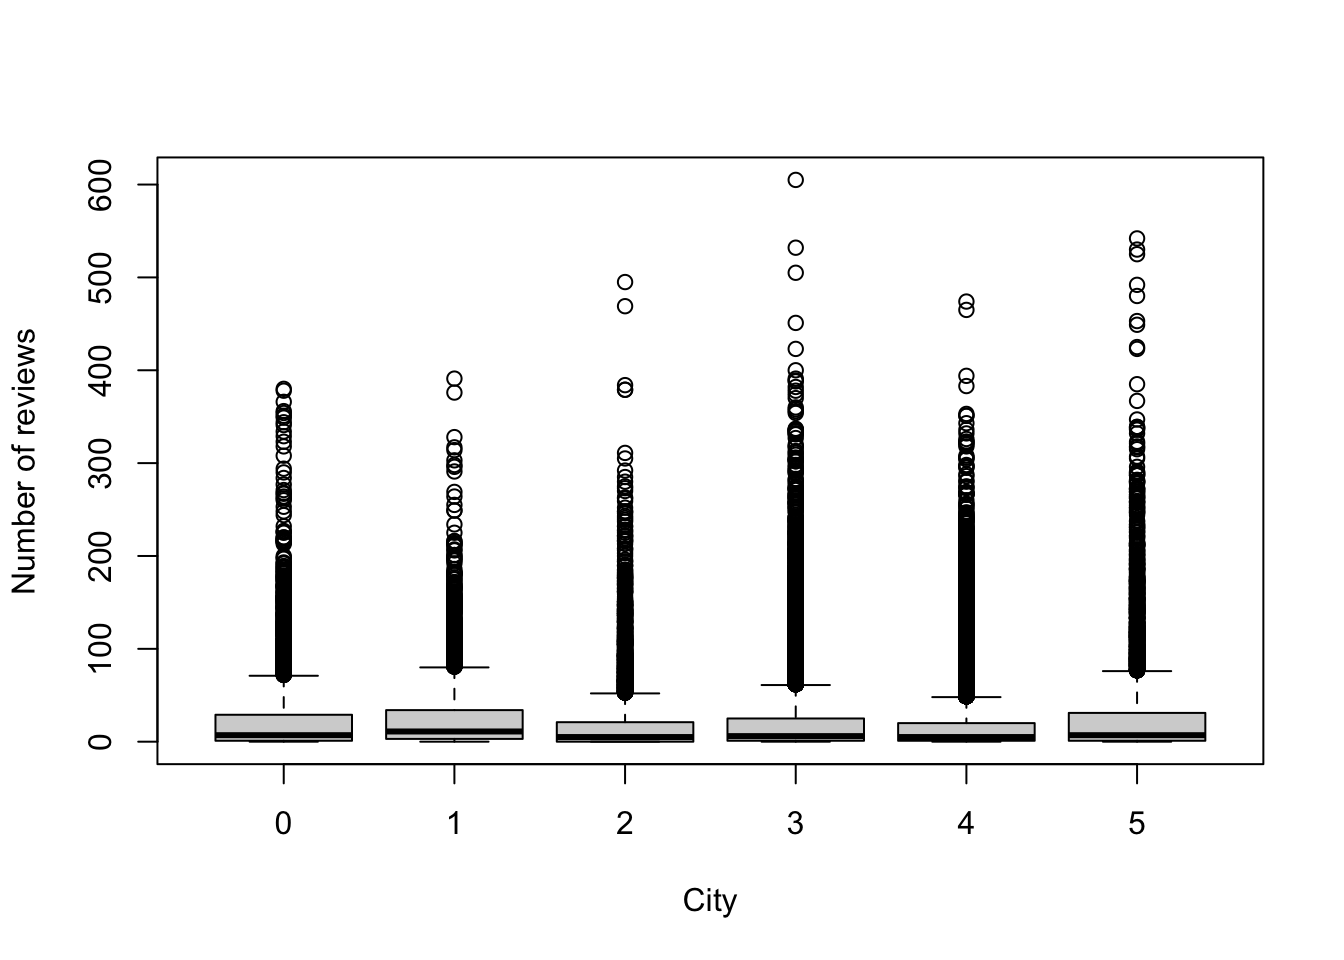
\includegraphics{R_Markdown_files/figure-latex/unnamed-chunk-7-1.pdf}

\begin{Shaded}
\begin{Highlighting}[]
\KeywordTok{boxplot}\NormalTok{(number_of_reviews }\OperatorTok{~}\StringTok{ }\NormalTok{room_type,}
        \DataTypeTok{ylab =} \StringTok{"Number of reviews"}\NormalTok{,}
        \DataTypeTok{xlab =} \StringTok{"Room type"}\NormalTok{,}
        \DataTypeTok{data =}\NormalTok{ df.airbnb)}
\end{Highlighting}
\end{Shaded}

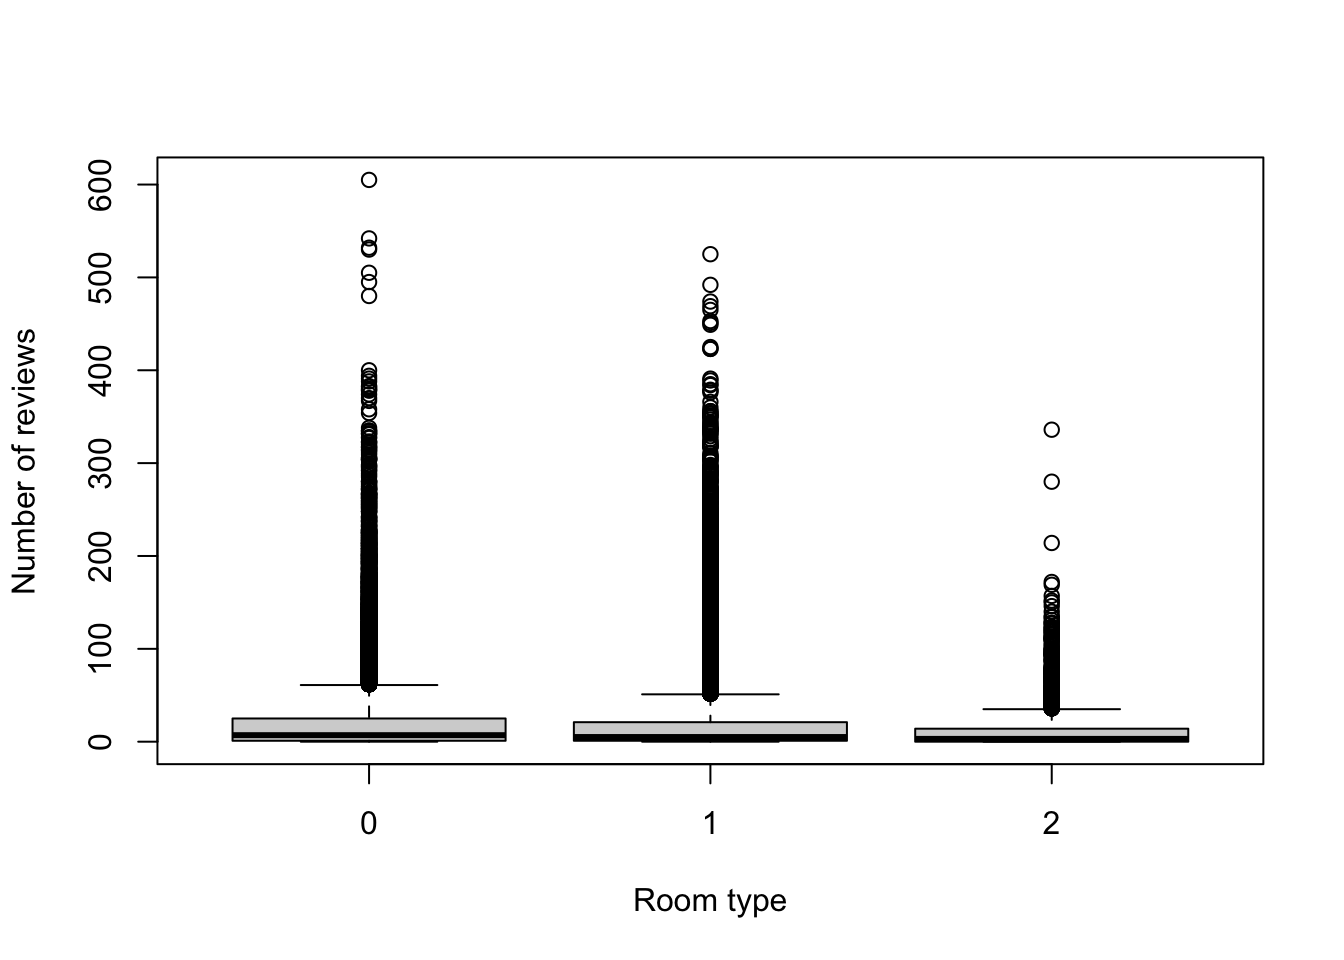
\includegraphics{R_Markdown_files/figure-latex/unnamed-chunk-7-2.pdf}

\begin{Shaded}
\begin{Highlighting}[]
\KeywordTok{boxplot}\NormalTok{(number_of_reviews }\OperatorTok{~}\StringTok{ }\NormalTok{property_type,}
        \DataTypeTok{ylab =} \StringTok{"Number of reviews"}\NormalTok{,}
        \DataTypeTok{xlab =} \StringTok{"Property type"}\NormalTok{,}
        \DataTypeTok{data =}\NormalTok{ df.airbnb)}
\end{Highlighting}
\end{Shaded}

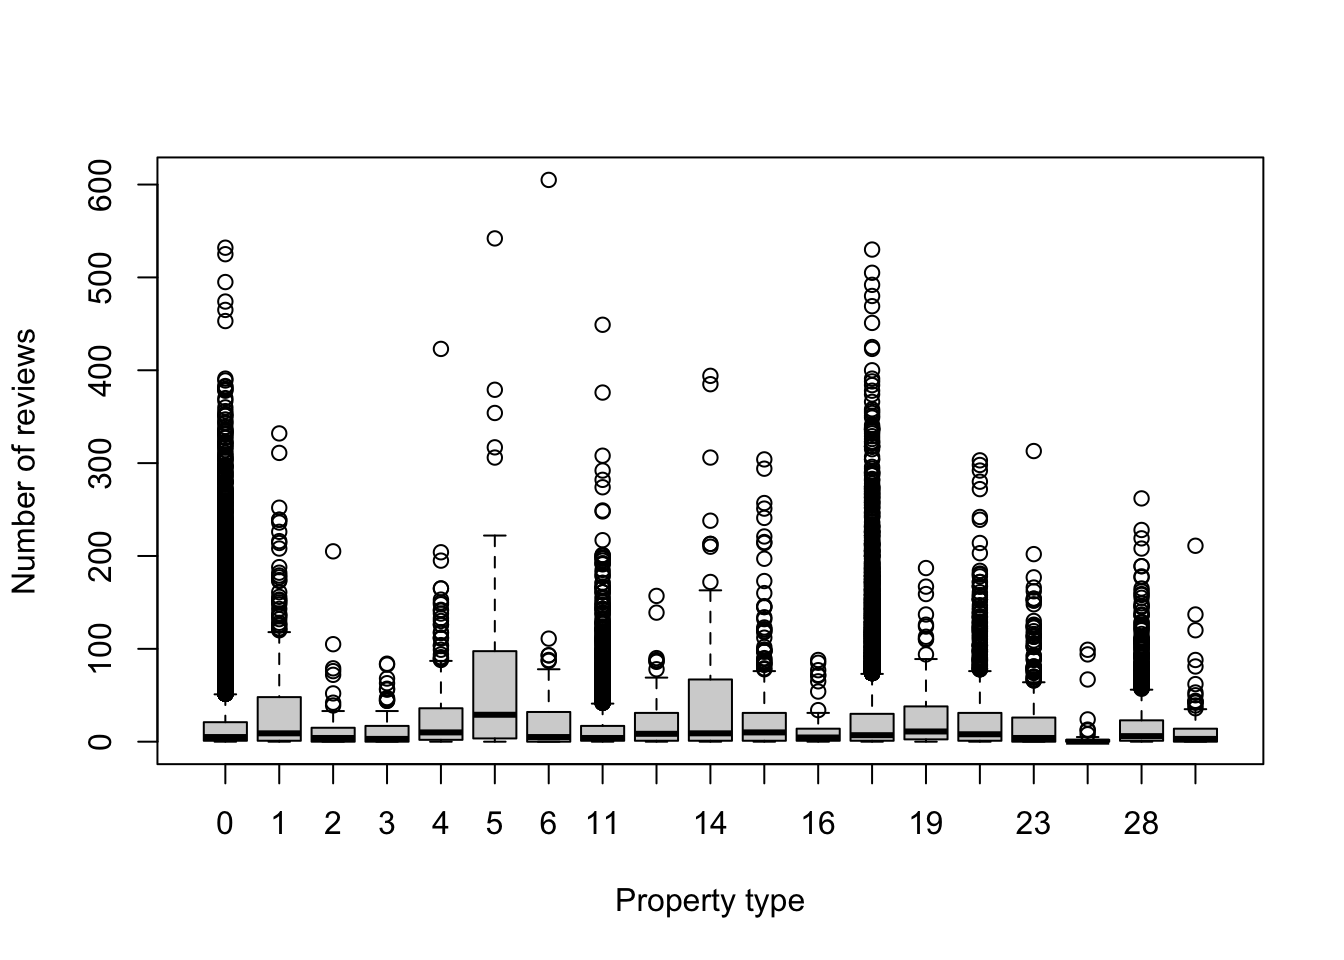
\includegraphics{R_Markdown_files/figure-latex/unnamed-chunk-7-3.pdf}

\begin{Shaded}
\begin{Highlighting}[]
\KeywordTok{plot}\NormalTok{(number_of_reviews }\OperatorTok{~}\StringTok{ }\NormalTok{review_scores_rating,}
        \DataTypeTok{ylab =} \StringTok{"Number of reviews"}\NormalTok{,}
        \DataTypeTok{xlab =} \StringTok{"Review scores"}\NormalTok{,}
        \DataTypeTok{data =}\NormalTok{ df.airbnb)}
\end{Highlighting}
\end{Shaded}

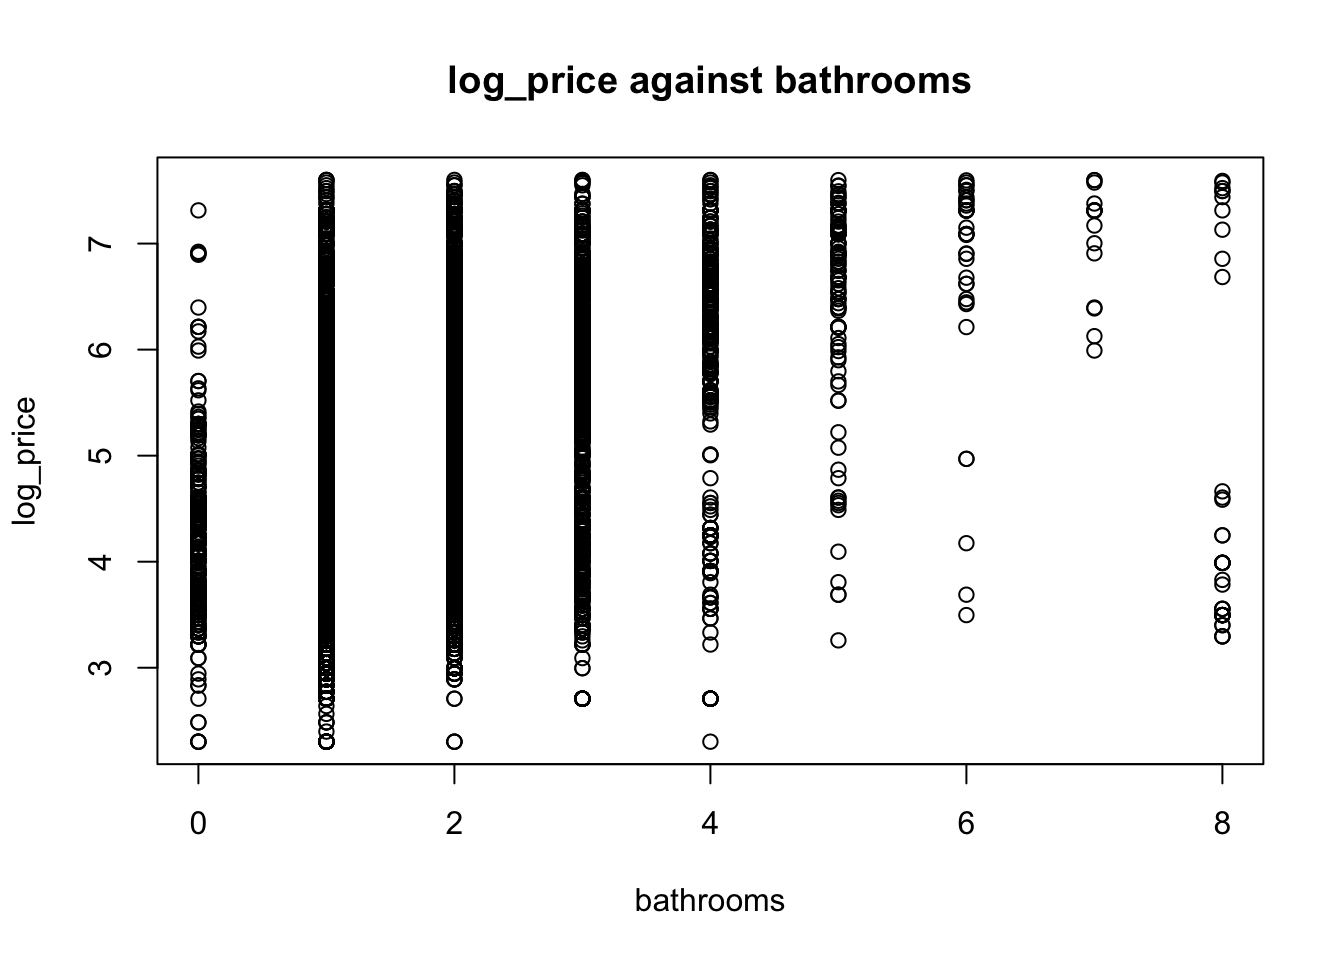
\includegraphics{R_Markdown_files/figure-latex/unnamed-chunk-7-4.pdf}

\begin{Shaded}
\begin{Highlighting}[]
\KeywordTok{plot}\NormalTok{(number_of_reviews }\OperatorTok{~}\StringTok{ }\NormalTok{log_price,}
        \DataTypeTok{ylab =} \StringTok{"Number of reviews"}\NormalTok{,}
        \DataTypeTok{xlab =} \StringTok{"log Price"}\NormalTok{,}
        \DataTypeTok{data =}\NormalTok{ df.airbnb)}
\end{Highlighting}
\end{Shaded}

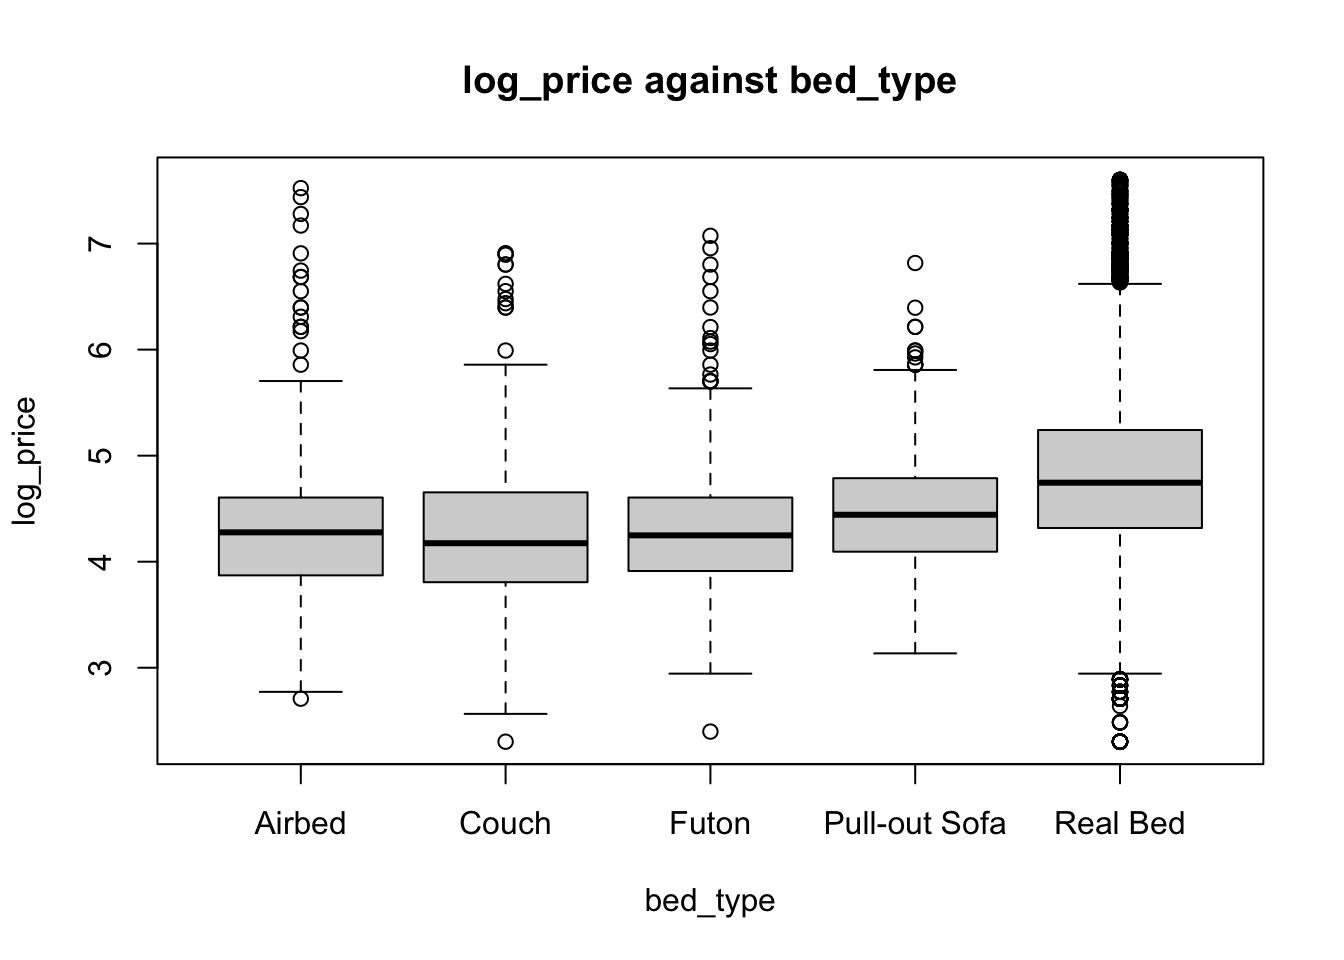
\includegraphics{R_Markdown_files/figure-latex/unnamed-chunk-7-5.pdf}

We can see that there is no clear evidence that the predictor ``City'',
``Room Type'' or ``Property Type'' have an influence on the response
variable. However, we could suggest a influence of the ``Review scores''
and the ``log Price''

Lets first create a simple model and a complex model. An see if the
predictors indicate evidence for an influence.

\begin{Shaded}
\begin{Highlighting}[]
\NormalTok{glm.df.airbnb}\FloatTok{.50}\NormalTok{ <-}\StringTok{ }\KeywordTok{glm}\NormalTok{(number_of_reviews }\OperatorTok{~}\StringTok{ }\NormalTok{city }\OperatorTok{+}\StringTok{ }\NormalTok{room_type }\OperatorTok{+}\StringTok{ }
\StringTok{                          }\NormalTok{review_scores_rating }\OperatorTok{+}\StringTok{ }\NormalTok{log_price }\OperatorTok{+}\StringTok{ }\NormalTok{property_type,}
                        \DataTypeTok{family =} \StringTok{"poisson"}\NormalTok{,}
                        \DataTypeTok{data =}\NormalTok{ df.airbnb)}
\KeywordTok{summary}\NormalTok{(glm.df.airbnb}\FloatTok{.50}\NormalTok{)}
\end{Highlighting}
\end{Shaded}

\begin{verbatim}
## 
## Call:
## glm(formula = number_of_reviews ~ city + room_type + review_scores_rating + 
##     log_price + property_type, family = "poisson", data = df.airbnb)
## 
## Deviance Residuals: 
##     Min       1Q   Median       3Q      Max  
## -13.150   -5.597   -3.804    0.541   52.605  
## 
## Coefficients:
##                        Estimate Std. Error  z value Pr(>|z|)    
## (Intercept)           4.3414882  0.0139582  311.035  < 2e-16 ***
## city1                -0.0398909  0.0046623   -8.556  < 2e-16 ***
## city2                -0.3045899  0.0045137  -67.481  < 2e-16 ***
## city3                -0.3116036  0.0037288  -83.568  < 2e-16 ***
## city4                -0.3518273  0.0036334  -96.831  < 2e-16 ***
## city5                 0.1354587  0.0041312   32.789  < 2e-16 ***
## room_type1           -0.2890526  0.0021585 -133.916  < 2e-16 ***
## room_type2           -0.8437048  0.0065127 -129.548  < 2e-16 ***
## review_scores_rating  0.0027494  0.0001227   22.401  < 2e-16 ***
## log_price            -0.2622712  0.0015546 -168.704  < 2e-16 ***
## property_type1        0.6381300  0.0082205   77.627  < 2e-16 ***
## property_type2       -0.2883463  0.0313127   -9.209  < 2e-16 ***
## property_type3       -0.3727183  0.0321550  -11.591  < 2e-16 ***
## property_type4        0.2915008  0.0101749   28.649  < 2e-16 ***
## property_type5        1.2667866  0.0136773   92.620  < 2e-16 ***
## property_type6        0.1657362  0.0205815    8.053 8.10e-16 ***
## property_type11      -0.2252135  0.0049342  -45.643  < 2e-16 ***
## property_type12       0.1434833  0.0196524    7.301 2.86e-13 ***
## property_type14       0.7058222  0.0131664   53.608  < 2e-16 ***
## property_type15       0.1875809  0.0090640   20.695  < 2e-16 ***
## property_type16      -0.1591918  0.0324103   -4.912 9.03e-07 ***
## property_type17       0.2680421  0.0020618  130.005  < 2e-16 ***
## property_type19       0.1430728  0.0209105    6.842 7.80e-12 ***
## property_type22       0.2704404  0.0059154   45.718  < 2e-16 ***
## property_type23       0.0304182  0.0092534    3.287  0.00101 ** 
## property_type26      -1.3757815  0.0517749  -26.572  < 2e-16 ***
## property_type28      -0.0043051  0.0058738   -0.733  0.46360    
## property_type32      -0.3406208  0.0217566  -15.656  < 2e-16 ***
## ---
## Signif. codes:  0 '***' 0.001 '**' 0.01 '*' 0.05 '.' 0.1 ' ' 1
## 
## (Dispersion parameter for poisson family taken to be 1)
## 
##     Null deviance: 3096713  on 73469  degrees of freedom
## Residual deviance: 2987584  on 73442  degrees of freedom
## AIC: 3230657
## 
## Number of Fisher Scoring iterations: 6
\end{verbatim}

We see that almost all predictors and factor levels seem to have some
sort of influence.

Lets create a more complex model and see the results.

\begin{Shaded}
\begin{Highlighting}[]
\NormalTok{glm.df.airbnb}\FloatTok{.51}\NormalTok{ <-}\KeywordTok{glm}\NormalTok{(number_of_reviews }\OperatorTok{~}\StringTok{ }\NormalTok{log_price }\OperatorTok{+}\StringTok{ }\NormalTok{property_type }\OperatorTok{+}\StringTok{ }\NormalTok{room_type }\OperatorTok{+}
\StringTok{                         }\NormalTok{accommodates }\OperatorTok{+}\StringTok{ }\NormalTok{bathrooms }\OperatorTok{+}\StringTok{ }\NormalTok{bed_type }\OperatorTok{+}\StringTok{ }\NormalTok{cancellation_policy }\OperatorTok{+}
\StringTok{                         }\NormalTok{cleaning_fee }\OperatorTok{+}\StringTok{ }\NormalTok{city }\OperatorTok{+}\StringTok{ }\NormalTok{host_has_profile_pic }\OperatorTok{+}
\StringTok{                         }\NormalTok{host_identity_verified }\OperatorTok{+}\StringTok{ }\NormalTok{instant_bookable }\OperatorTok{+}
\StringTok{                         }\NormalTok{review_scores_rating }\OperatorTok{+}\StringTok{ }\NormalTok{bedrooms }\OperatorTok{+}\StringTok{ }\NormalTok{beds }\OperatorTok{+}\StringTok{ }\NormalTok{amenities_Breakfast }\OperatorTok{+}
\StringTok{                         }\NormalTok{amenities_Gym }\OperatorTok{+}\StringTok{ }\NormalTok{amenities_Pets }\OperatorTok{+}\StringTok{ }\NormalTok{amenities_WiFi,}
                        \DataTypeTok{family =} \StringTok{"quasipoisson"}\NormalTok{,}
                        \DataTypeTok{data =}\NormalTok{ df.airbnb)}
\KeywordTok{summary}\NormalTok{(glm.df.airbnb}\FloatTok{.51}\NormalTok{)}
\end{Highlighting}
\end{Shaded}

\begin{verbatim}
## 
## Call:
## glm(formula = number_of_reviews ~ log_price + property_type + 
##     room_type + accommodates + bathrooms + bed_type + cancellation_policy + 
##     cleaning_fee + city + host_has_profile_pic + host_identity_verified + 
##     instant_bookable + review_scores_rating + bedrooms + beds + 
##     amenities_Breakfast + amenities_Gym + amenities_Pets + amenities_WiFi, 
##     family = "quasipoisson", data = df.airbnb)
## 
## Deviance Residuals: 
##     Min       1Q   Median       3Q      Max  
## -17.301   -4.764   -2.912    0.449   49.839  
## 
## Coefficients:
##                           Estimate Std. Error t value Pr(>|t|)    
## (Intercept)              1.1148502  0.2426876   4.594 4.36e-06 ***
## log_price               -0.1928356  0.0139741 -13.800  < 2e-16 ***
## property_type1           0.7105151  0.0625401  11.361  < 2e-16 ***
## property_type2           0.0763579  0.2336416   0.327 0.743808    
## property_type3          -0.1299181  0.2399677  -0.541 0.588235    
## property_type4           0.1724469  0.0759249   2.271 0.023133 *  
## property_type5           1.2636854  0.1020401  12.384  < 2e-16 ***
## property_type6           0.3512676  0.1538194   2.284 0.022396 *  
## property_type11         -0.2154747  0.0368406  -5.849 4.97e-09 ***
## property_type12         -0.0463802  0.1494252  -0.310 0.756265    
## property_type14          0.5751335  0.0981427   5.860 4.64e-09 ***
## property_type15          0.0551062  0.0676922   0.814 0.415607    
## property_type16         -0.4574452  0.2449554  -1.867 0.061841 .  
## property_type17          0.2206361  0.0161065  13.699  < 2e-16 ***
## property_type19          0.0048548  0.1558009   0.031 0.975142    
## property_type22          0.1282283  0.0443404   2.892 0.003830 ** 
## property_type23         -0.0357981  0.0693546  -0.516 0.605744    
## property_type26         -1.2508359  0.3858419  -3.242 0.001188 ** 
## property_type28         -0.0968076  0.0440097  -2.200 0.027832 *  
## property_type32         -0.4185557  0.1622129  -2.580 0.009874 ** 
## room_type1              -0.0016870  0.0170689  -0.099 0.921269    
## room_type2              -0.4430071  0.0509518  -8.695  < 2e-16 ***
## accommodates             0.0715001  0.0051255  13.950  < 2e-16 ***
## bathrooms               -0.1484697  0.0159140  -9.329  < 2e-16 ***
## bed_type1                0.0733821  0.1591725   0.461 0.644784    
## bed_type2                0.4475284  0.1063964   4.206 2.60e-05 ***
## bed_type3                0.3788179  0.1108793   3.416 0.000635 ***
## bed_type4                0.1839934  0.0926301   1.986 0.047001 *  
## cancellation_policy1     0.9099577  0.0207474  43.859  < 2e-16 ***
## cancellation_policy2     0.9728447  0.0199035  48.878  < 2e-16 ***
## cancellation_policy3     0.1537721  0.2355679   0.653 0.513905    
## cancellation_policy4    -0.4819886  0.9315112  -0.517 0.604860    
## cleaning_fee1            0.0969222  0.0167578   5.784 7.34e-09 ***
## city1                   -0.0939789  0.0350651  -2.680 0.007361 ** 
## city2                   -0.2444814  0.0337754  -7.238 4.58e-13 ***
## city3                   -0.2912248  0.0279322 -10.426  < 2e-16 ***
## city4                   -0.3447008  0.0271698 -12.687  < 2e-16 ***
## city5                    0.1192507  0.0310304   3.843 0.000122 ***
## host_has_profile_pic1    0.4062825  0.1881381   2.159 0.030815 *  
## host_identity_verified1  0.5758118  0.0156914  36.696  < 2e-16 ***
## instant_bookable1        0.2986337  0.0131079  22.783  < 2e-16 ***
## review_scores_rating     0.0033204  0.0009654   3.439 0.000583 ***
## bedrooms                -0.2355124  0.0113031 -20.836  < 2e-16 ***
## beds                     0.0563260  0.0079321   7.101 1.25e-12 ***
## amenities_Breakfast1    -0.0726376  0.0199463  -3.642 0.000271 ***
## amenities_Gym1          -0.3628328  0.0244234 -14.856  < 2e-16 ***
## amenities_Pets1         -0.0036701  0.0177002  -0.207 0.835737    
## amenities_WiFi1          0.9770272  0.0606549  16.108  < 2e-16 ***
## ---
## Signif. codes:  0 '***' 0.001 '**' 0.01 '*' 0.05 '.' 0.1 ' ' 1
## 
## (Dispersion parameter for quasipoisson family taken to be 55.46548)
## 
##     Null deviance: 3096713  on 73469  degrees of freedom
## Residual deviance: 2520001  on 73422  degrees of freedom
## AIC: NA
## 
## Number of Fisher Scoring iterations: 6
\end{verbatim}

Again, most of the predictors have an influence, let's ensure this even
further.

\begin{Shaded}
\begin{Highlighting}[]
\KeywordTok{drop1}\NormalTok{(glm.df.airbnb}\FloatTok{.51}\NormalTok{, }\DataTypeTok{test =} \StringTok{"F"}\NormalTok{)}
\end{Highlighting}
\end{Shaded}

\begin{verbatim}
## Single term deletions
## 
## Model:
## number_of_reviews ~ log_price + property_type + room_type + accommodates + 
##     bathrooms + bed_type + cancellation_policy + cleaning_fee + 
##     city + host_has_profile_pic + host_identity_verified + instant_bookable + 
##     review_scores_rating + bedrooms + beds + amenities_Breakfast + 
##     amenities_Gym + amenities_Pets + amenities_WiFi
##                        Df Deviance   F value    Pr(>F)    
## <none>                     2520001                        
## log_price               1  2530702  311.7882 < 2.2e-16 ***
## property_type          18  2549115   47.1254 < 2.2e-16 ***
## room_type               2  2525144   74.9175 < 2.2e-16 ***
## accommodates            1  2529989  291.0182 < 2.2e-16 ***
## bathrooms               1  2525052  147.1542 < 2.2e-16 ***
## bed_type                4  2522021   14.7107 5.133e-12 ***
## cancellation_policy     4  2686790 1214.8776 < 2.2e-16 ***
## cleaning_fee            1  2521888   54.9695 1.237e-13 ***
## city                    5  2553228  193.6154 < 2.2e-16 ***
## host_has_profile_pic    1  2520298    8.6495  0.003272 ** 
## host_identity_verified  1  2603033 2419.2055 < 2.2e-16 ***
## instant_bookable        1  2547806  810.1096 < 2.2e-16 ***
## review_scores_rating    1  2520673   19.5704 9.710e-06 ***
## bedrooms                1  2543692  690.2617 < 2.2e-16 ***
## beds                    1  2522721   79.2482 < 2.2e-16 ***
## amenities_Breakfast     1  2520750   21.8123 3.012e-06 ***
## amenities_Gym           1  2533434  391.3757 < 2.2e-16 ***
## amenities_Pets          1  2520003    0.0695  0.792014    
## amenities_WiFi          1  2539981  582.1434 < 2.2e-16 ***
## ---
## Signif. codes:  0 '***' 0.001 '**' 0.01 '*' 0.05 '.' 0.1 ' ' 1
\end{verbatim}

Apart from the preditcor ``amenities\_Pets'' all predictors seem to have
an influence, hence our final model will use all predictors except the
one mentioned before.

\begin{Shaded}
\begin{Highlighting}[]
\NormalTok{glm.df.airbnb}\FloatTok{.52}\NormalTok{ <-}\StringTok{ }\KeywordTok{update}\NormalTok{(glm.df.airbnb}\FloatTok{.51}\NormalTok{, . }\OperatorTok{~}\StringTok{ }\NormalTok{. }\OperatorTok{-}\StringTok{ }\NormalTok{amenities_Pets)}
\end{Highlighting}
\end{Shaded}

Additionally, we will create a GAM model to account for non-linerar
relationships of the two contiuous predictors ``log\_price'' and
``review\_scores\_rating''.

\begin{Shaded}
\begin{Highlighting}[]
\NormalTok{gam.df.airbnb}\FloatTok{.53}\NormalTok{ <-}\StringTok{ }\KeywordTok{gam}\NormalTok{(number_of_reviews }\OperatorTok{~}\StringTok{ }\KeywordTok{s}\NormalTok{(log_price) }\OperatorTok{+}\StringTok{ }\NormalTok{property_type }\OperatorTok{+}\StringTok{ }\NormalTok{room_type }\OperatorTok{+}
\StringTok{                          }\NormalTok{accommodates }\OperatorTok{+}\StringTok{ }\NormalTok{bathrooms }\OperatorTok{+}\StringTok{ }\NormalTok{bed_type }\OperatorTok{+}\StringTok{ }\NormalTok{cancellation_policy }\OperatorTok{+}
\StringTok{                          }\NormalTok{cleaning_fee }\OperatorTok{+}\StringTok{ }\NormalTok{city }\OperatorTok{+}\StringTok{ }\NormalTok{host_has_profile_pic }\OperatorTok{+}
\StringTok{                          }\NormalTok{host_identity_verified }\OperatorTok{+}\StringTok{ }\NormalTok{instant_bookable }\OperatorTok{+}
\StringTok{                          }\KeywordTok{s}\NormalTok{(review_scores_rating) }\OperatorTok{+}\StringTok{ }\NormalTok{bedrooms }\OperatorTok{+}\StringTok{ }\NormalTok{beds }\OperatorTok{+}\StringTok{ }
\StringTok{                          }\NormalTok{amenities_Breakfast }\OperatorTok{+}\StringTok{ }\NormalTok{amenities_Gym }\OperatorTok{+}\StringTok{ }\NormalTok{amenities_WiFi,}
                        \DataTypeTok{family =} \StringTok{"quasipoisson"}\NormalTok{,}
                        \DataTypeTok{data =}\NormalTok{ df.airbnb)}
\end{Highlighting}
\end{Shaded}

To check which model fits better, we will run a 10-fold cross validation
check.

\begin{Shaded}
\begin{Highlighting}[]
\KeywordTok{set.seed}\NormalTok{(}\DecValTok{544}\NormalTok{)}
\NormalTok{r.squared.simple <-}\StringTok{ }\KeywordTok{c}\NormalTok{()}
\NormalTok{r.squared.complex <-}\StringTok{ }\KeywordTok{c}\NormalTok{()}
\CommentTok{# shuffle data}
\NormalTok{df.airbnb <-}\StringTok{ }\NormalTok{df.airbnb[}\KeywordTok{sample}\NormalTok{(}\KeywordTok{nrow}\NormalTok{(df.airbnb)),]}
\NormalTok{folds <-}\StringTok{ }\KeywordTok{cut}\NormalTok{(}\KeywordTok{seq}\NormalTok{(}\DecValTok{1}\NormalTok{,}\KeywordTok{nrow}\NormalTok{(df.airbnb)), }\DataTypeTok{breaks =} \DecValTok{10}\NormalTok{, }\DataTypeTok{labels =} \OtherTok{FALSE}\NormalTok{)}
\ControlFlowTok{for}\NormalTok{(i }\ControlFlowTok{in} \DecValTok{1}\OperatorTok{:}\DecValTok{10}\NormalTok{)\{}
\NormalTok{  testIndexes <-}\StringTok{ }\KeywordTok{which}\NormalTok{(folds}\OperatorTok{==}\NormalTok{i, }\DataTypeTok{arr.ind =} \OtherTok{TRUE}\NormalTok{)}
\NormalTok{  df.airbnb.test <-}\StringTok{ }\NormalTok{df.airbnb[testIndexes, ]}
\NormalTok{  df.airbnb.train <-}\StringTok{ }\NormalTok{df.airbnb[}\OperatorTok{-}\NormalTok{testIndexes, ]}
  \CommentTok{## insert your models - simple}
  \CommentTok{# fit the model with test data}
\NormalTok{  model.}\FloatTok{1.}\NormalTok{train <-}\StringTok{ }\KeywordTok{glm}\NormalTok{(}\DataTypeTok{formula =} \KeywordTok{formula}\NormalTok{(glm.df.airbnb}\FloatTok{.52}\NormalTok{),}
                       \DataTypeTok{data =}\NormalTok{ df.airbnb.train)}
  \CommentTok{# predict the model}
\NormalTok{  predicted.model.}\FloatTok{1.}\NormalTok{test <-}\StringTok{ }\KeywordTok{predict}\NormalTok{(model.}\FloatTok{1.}\NormalTok{train,}
                                    \DataTypeTok{newdata =}\NormalTok{ df.airbnb.test)}
  \CommentTok{# compute R^2}
\NormalTok{  r.squared.simple[i] <-}\StringTok{ }\KeywordTok{cor}\NormalTok{(predicted.model.}\FloatTok{1.}\NormalTok{test, }
\NormalTok{                             df.airbnb.test}\OperatorTok{$}\NormalTok{number_of_reviews)}\OperatorTok{^}\DecValTok{2}
  \CommentTok{## insert you model - complex}
  \CommentTok{# fit the model with test data}
\NormalTok{  model.}\FloatTok{2.}\NormalTok{train <-}\StringTok{ }\KeywordTok{gam}\NormalTok{(}\DataTypeTok{formula =} \KeywordTok{formula}\NormalTok{(gam.df.airbnb}\FloatTok{.53}\NormalTok{),}
                       \DataTypeTok{data =}\NormalTok{ df.airbnb.train)}
  \CommentTok{# predict the model}
\NormalTok{  predicted.model.}\FloatTok{2.}\NormalTok{test <-}\StringTok{ }\KeywordTok{predict}\NormalTok{(model.}\FloatTok{2.}\NormalTok{train,}
                                    \DataTypeTok{newdata =}\NormalTok{ df.airbnb.test)}
  \CommentTok{# compute R^2}
\NormalTok{  r.squared.complex[i] <-}\StringTok{ }\KeywordTok{cor}\NormalTok{(predicted.model.}\FloatTok{2.}\NormalTok{test, }
\NormalTok{                           df.airbnb.test}\OperatorTok{$}\NormalTok{number_of_reviews)}\OperatorTok{^}\DecValTok{2}
\NormalTok{\}}
\end{Highlighting}
\end{Shaded}

\begin{Shaded}
\begin{Highlighting}[]
\KeywordTok{print}\NormalTok{(}\KeywordTok{mean}\NormalTok{(r.squared.simple)}\OperatorTok{*}\DecValTok{100}\NormalTok{)}
\end{Highlighting}
\end{Shaded}

\begin{verbatim}
## [1] 10.22684
\end{verbatim}

\begin{Shaded}
\begin{Highlighting}[]
\KeywordTok{print}\NormalTok{(}\KeywordTok{mean}\NormalTok{(r.squared.complex)}\OperatorTok{*}\DecValTok{100}\NormalTok{)}
\end{Highlighting}
\end{Shaded}

\begin{verbatim}
## [1] 12.50048
\end{verbatim}

From the results we can see, the GAM model fits better and should
therefore be considered. However, the result is not great and more
predictors should be evaluated to come up with a better model.

\hypertarget{applying-the-binomial-distribution}{%
\subsection{Applying the Binomial
Distribution}\label{applying-the-binomial-distribution}}

\hypertarget{applying-a-gam}{%
\subsection{Applying a GAM}\label{applying-a-gam}}

\hypertarget{using-the-support-vector-machines}{%
\subsection{Using the Support Vector
Machines}\label{using-the-support-vector-machines}}

\hypertarget{using-a-neural-network}{%
\subsection{Using a Neural Network}\label{using-a-neural-network}}

\hypertarget{using-an-approximate-bayesian-computation}{%
\subsection{Using an Approximate Bayesian
Computation}\label{using-an-approximate-bayesian-computation}}

\hypertarget{comparing-the-best-models-of-each-class}{%
\subsection{Comparing the best Models of each
Class}\label{comparing-the-best-models-of-each-class}}

\hypertarget{conclusion-and-model-selection}{%
\section{Conclusion and Model
Selection}\label{conclusion-and-model-selection}}

\end{document}
